% +--------------------------------------------------------------------+
% | Sample Chapter 2
% +--------------------------------------------------------------------+

\cleardoublepage

% +--------------------------------------------------------------------+
% | Replace "This is Chapter 2" below with the title of your chapter.
% | LaTeX will automatically number the chapters.
% +--------------------------------------------------------------------+

\chapter{State of the Art}
\label{makereference2}

This chapter expose the current state of Edge computing related to Internet of Things. Different types of architectures that diverge in core technologies regarding edge environments are going to be disccussed,  also we'll cover some projects that provide \textit{similar} solutions to Epfiot.

Chapter ~\ref{makereference} has covered some basic definitions used in the project such as Virtualization, however this is not the only option regarding technologies that allow to prepare the proper infraestructure in a edge context.

\section{Containers, lightweight alternative}
\label{makereference2.1}

Virtualization has been around for a long time but since a few years ago, containers were adopted globally transforming the IT world
as we know it.

A \textbf{Container} is a set of one or more process that are isolated from the rest of the operating system, these process lately would be very useful to prepare independent components that share resources with the host machine and have portability. 
Containers are a form of virtualization, while virtualization work at hardware level emulating all the resources that are needed for a guest operating system to run, containers in the other hand work at operating system level being a lightweight alternative.

The idea of the container technology appeared in 2000 as FreeBSD jail, safe environment that a system administrator could share with multiple users. Later more technologies combined to make this isolated approach a reality, for example Control groups is a kernel feature that controls and limits resource usage for a process or groups of processes or systemd, an initialization system that sets up the userspace and manages their processes. In 2008 Docker was born with a new container technology adding new concepts and tools, layered images, command line tools, a server daemon granting to the user the ability of build new containers quickly and share between others.~\cite{redhat_container}

\begin{figure}[h!]%t=top, b=bottom, h=here
    \centering
    
\includegraphics[width=2.5in]{figures/docker.png}
~\caption{docker container logo}
\label{figure2.1}
\end{figure}

\section{Virtualization and Containers, what to choose}
\label{makereference2.2}

The infrastructure takes into account several factors.

\begin{itemize}
    \item System software that is going to run at the top of the architecture fast and lightweight. Designed to operate directly on edge devices (computation, network, storage) and for this purpose, normally system software needs the support of multi-tenancy and isolation.
    \item Resource constrained because edge devices have smaller processors and limited power budget ~\ref{makereference1.1}, managing these resources properly is one of the challenge that edge computing need to confront.
    \item Elastic scalation, depending on the services that are going to be provided.
    \item Network capabilities
\end{itemize}
In a edge computing scenario is usually to see several applications running from differents tenants, knowing the factors previously discussed both containers and virtual machines are valid approaches in order to satisfy the edge requirements.~\cite{CORR:chong:2018} Both enable fault and performacne isolation beetween tenants and limits and accounts for the resource usage.
\newpage

However there are differences, see figure \ref{figure2.2}.

\begin{itemize}
  \item Virtual Machines are built including virtualized resources that emulate the entire computer such as  CPU, memory, network, storage, gpu... This means that the tenant install the operating system and runs applications like in a real psysical machine. Virtualization isolates completly the execution environment.
  \item Containers are lightweight virtualization and are multiplexed by a single linux kernel, they don't require an additional layer if you compare them with the virtual machines, share same OS kernel keeping the isolation principles using cgroups and Linux namespaces allowing the containers to achieve performance similiar to that of the native environment.
\end{itemize}

\begin{figure}[h]%t=top, b=bottom, h=here
% \centering
    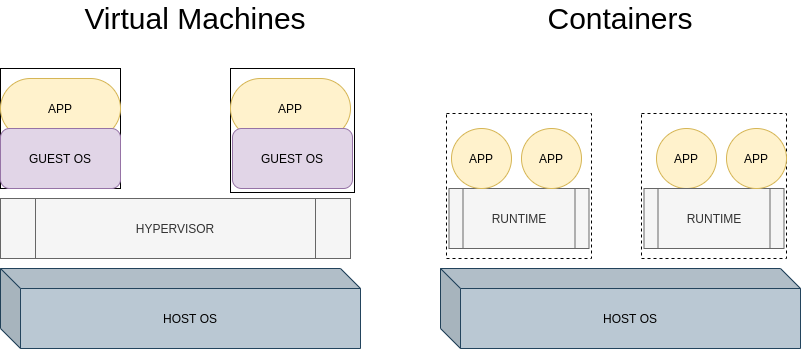
\includegraphics[width=6.5in]{figures/virt_container.png}
~\caption{virtual machine architecture and container architecure}
\label{figure2.2}
\end{figure}

Choose what kind of technology is better in a edge environment is not an easy question, virtualization approaches varies from system to system. Many recent works chose lightweight OS-Level virtualization like LXC to run services on edge systems that have limited storage and processing capabilities, unlike virtual machines, multiple containers share the same Linux kernel and therefore exhibit very small overhead.~\cite{ACM:clixue:2018}



Taking into account the lightweight capability of the containers reducing resource comsumition it could be said that is the perfect solution for Edge computing, however it faces serious security problems that are solved in a virtual machine architecture. 

\newpage

In order to compare both technologies, a table has been provides, see table \ref{table1}.

\begin{table}
% +--------------------------------------------------------------------+
% | We include the command \begin{center} to center the table
% | horizontally on the page.  Note use of the command \end{center}
% | to turn off centering after the table is defined.
% +--------------------------------------------------------------------+
    \begin{center}
% +--------------------------------------------------------------------+
% | The table is created with this command
% |
% | \begin{tabular}[pos]{table spec}
% |
% | The "pos" argument specifies the vertical position of the table relative to
% | the baseline of the surrounding text.  Use t, b, or c to specify alignment
% | at the top, bottom, or center.
% |
% | The "table spec" command defines the format of the table
% |   l for a column of left-aligned text
% |   r for a column of right-aligned text
% |   c for centered text
% |   p{width} for a column containing justified text with line breaks
% |   | for a vertical line
% +--------------------------------------------------------------------+
    \begin{tabular}[h]{|c|c|}
        \hline
        \textbf{Virtual Machines} & \textbf{Containers}\\
        \hline
        Heavyweight & Lightweigh\\
        Each VM runs in its own OS	 & All containers share the host OS\\
        Hardware-level virtualization & OS virtualization \\
        Startup time in minutes	 & Startup time in milliseconds \\
        Allocates required memory & Requires less memory space \\
        Fully isolated and hence more secure & Process-level isolation, possibly less secure\\
        \hline
    \end{tabular}
    \caption{vms and container comparison. ~\cite{virt_comparison}}
    \label{table1}
   \end{center}
\end{table}


Security issues is one of the most important things to take into account, however containers are lightweigh, have better startup time and the resource requirements are by far better taking considerations that we are in a edge environment and all that his implies, important factors defined in ~\ref{makereference2.2}

However EPFIOT project takes that into account and with the new forms of virtualization there are some key features that could be improved:
\begin{itemize}
    \item Baremetal performance using Linux hypervisor
    \item hardware passthrough
    \item lightweight vm images
\end{itemize}

These features balance both technologies, on an edge approach it would be better to use containers if the service require a high level scalation on demand and the security issues are covered, but in a scenareo that do not require this high elastic scalation and some third party hardware is being used (usb acceleators), a virtualization approach would be a better fit, taking into account that usually you need concrete hardware requirements to meet with the third party hardware provider.

\newpage
